\documentclass[a4paper]{article}
\usepackage{amsfonts}
\usepackage{amsmath}
\usepackage{amssymb}
\usepackage{graphicx}
\usepackage{float}

\begin{document}
  
\noindent \large Auteur: Siebe Mees \\
\noindent \large Studierichting: Informatica\\
\noindent \large Oefeningenreeks 5D nr. 1.8\\

\medskip

\normalsize

$f(x)=\cos x - \sin x $ op $ \left[0,\dfrac{\pi}{4}\right]$\\

$\displaystyle\int_{0}^{\tfrac{\pi}{4}} (\cos x - \sin x) dx$\\

$= \left[ \sin x + \cos x \right]_{0}^{\tfrac{\pi}{4}}$\\

$= \left( \sin \dfrac{\pi}{4} + \cos \dfrac{\pi}{4} \right) - \left( \sin 0 + \cos 0 \right)$\\

$= \left( \dfrac{\sqrt{2}}{2} + \dfrac{\sqrt{2}}{2} \right) - (0 + 1)$\\

$= \sqrt{2} - 1$\\


$\Rightarrow \text{Tekening}$\\

\begin{tabular}{c|cc}

$x$ & $0$ & $\dfrac{\pi}{4}$ \\ \hline

$f(x)$ & $1$ & $0$ \\

$f'(x)$ & $-$ & $-$ \\

$f''(x)$ & $-$ & $0$ \\ \hline

$f(x)$ & $\searrow$ & $\searrow$ \\

& $\frown$ & $\frown$ \\

\end{tabular}\\

\begin{figure}[H]
\centering
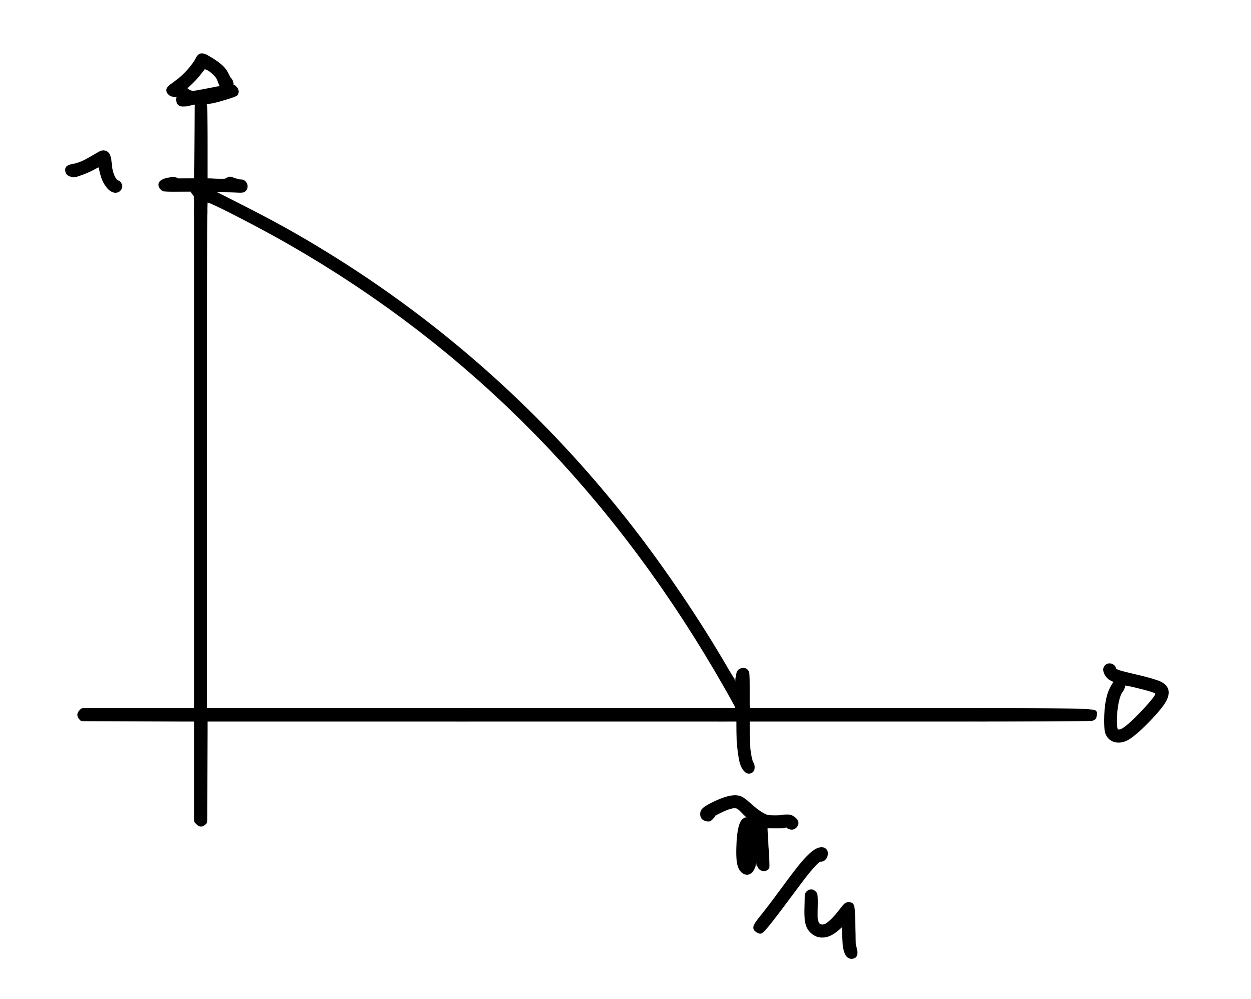
\includegraphics[width=5cm]{5D-1.8-siebe.mees.INF.png}
\end{figure}

\begin{thebibliography}{999}
%\bibitem{a} Referentie
\end{thebibliography}
\end{document} 
